
%%%%%%%%%%%%%%%%%%%%%%%%%%%%%%%%%%%%%%%%%
% Short Sectioned Assignment LaTeX Template Version 1.0 (5/5/12)
% This template has been downloaded from: http://www.LaTeXTemplates.com
% Original author:  Frits Wenneker (http://www.howtotex.com)
% License: CC BY-NC-SA 3.0 (http://creativecommons.org/licenses/by-nc-sa/3.0/)
%%%%%%%%%%%%%%%%%%%%%%%%%%%%%%%%%%%%%%%%%

%----------------------------------------------------------------------------------------
%	PACKAGES AND OTHER DOCUMENT CONFIGURATIONS
%----------------------------------------------------------------------------------------

\documentclass[paper=a4, fontsize=11pt]{scrartcl} % A4 paper and 11pt font size

% ---- Entrada y salida de texto -----

\usepackage[T1]{fontenc} % Use 8-bit encoding that has 256 glyphs
\usepackage[utf8]{inputenc}
%\usepackage{fourier} % Use the Adobe Utopia font for the document - comment this line to return to the LaTeX default

% ---- Idioma --------

\usepackage[spanish, es-tabla]{babel} % Selecciona el español para palabras introducidas automáticamente, p.ej. "septiembre" en la fecha y especifica que se use la palabra Tabla en vez de Cuadro

% ---- Otros paquetes ----

\usepackage{url} % ,href} %para incluir URLs e hipervínculos dentro del texto (aunque hay que instalar href)
\usepackage{amsmath,amsfonts,amsthm} % Math packages
%\usepackage{graphics,graphicx, floatrow} %para incluir imágenes y notas en las imágenes
\usepackage{graphics,graphicx, float} %para incluir imágenes y colocarlas
\usepackage{subfigure} % subfiguras

% Para hacer tablas comlejas
%\usepackage{multirow}
%\usepackage{threeparttable}

%\usepackage{sectsty} % Allows customizing section commands
%\allsectionsfont{\centering \normalfont\scshape} % Make all sections centered, the default font and small caps

\usepackage{fancyhdr} % Custom headers and footers
\usepackage{pdflscape}

\pagestyle{fancyplain} % Makes all pages in the document conform to the custom headers and footers
\fancyhead{} % No page header - if you want one, create it in the same way as the footers below
\fancyfoot[L]{} % Empty left footer
\fancyfoot[C]{} % Empty center footer
\fancyfoot[R]{\thepage} % Page numbering for right footer
\renewcommand{\headrulewidth}{0pt} % Remove header underlines
\renewcommand{\footrulewidth}{0pt} % Remove footer underlines
\setlength{\headheight}{13.6pt} % Customize the height of the header

\numberwithin{equation}{section} % Number equations within sections (i.e. 1.1, 1.2, 2.1, 2.2 instead of 1, 2, 3, 4)
\numberwithin{figure}{section} % Number figures within sections (i.e. 1.1, 1.2, 2.1, 2.2 instead of 1, 2, 3, 4)
\numberwithin{table}{section} % Number tables within sections (i.e. 1.1, 1.2, 2.1, 2.2 instead of 1, 2, 3, 4)


\setlength\parindent{0pt} % Removes all indentation from paragraphs - comment this line for an assignment with lots of text

\newcommand{\horrule}[1]{\rule{\linewidth}{#1}} % Create horizontal rule command with 1 argument of height
\usepackage[breaklinks=true]{hyperref}

\usepackage[dvipsnames]{xcolor}
\usepackage{amssymb}
\usepackage{color}
\usepackage{listings}
\usepackage{upgreek} % para poner letras griegas sin cursiva
\usepackage{cancel} % para tachar
\usepackage{mathdots} % para el comando \iddots
\usepackage{mathrsfs} % para formato de letra
\usepackage{stackrel} % para el comando \stackbin
\lstset{ %
language=C++,                % elegir el lenguaje del código
stringstyle=\color{blue}\ttfamily,,
basicstyle=\normalsize\ttfamily,       % el tamaño del font a usar para el código
numbers=left,                   % dónde poner los números de línea 
numberstyle=\footnotesize,      % tamaño de font usados para los números de línea 
stepnumber=1,                   % el paso de numeración
numbersep=5pt,                  % distancia del numero de línea y la línea
backgroundcolor=\color{white},  % color de fondo, para usarlo hay que agregar  \usepackage{color}
showspaces=false,               % mostrar espacios en blanco ?
showstringspaces=false,         % subrayar espacios con cadenas?   
 showtabs=false,                 % mostrar taba usando cadenas? 
frame=single,           			% enmarcar el código?  
tabsize=2,          				% sets default tabsize to 2 spaces?
keywordstyle=\color{MidnightBlue}\ttfamily\bfseries,
commentstyle=\color{OliveGreen}\ttfamily,
morecomment=[l][\color{OliveGreen}]{\#},
captionpos=b,           % sets the caption-position to bottom?
breaklines=true,        % sets automatic line breaking?
breakatwhitespace=false,    % sets if automatic breaks should only happen at whitespace ?
title=\lstname,
escapeinside={\%*}{*)}          % if you want to add a comment within your code
}

\lstset{literate=
  {á}{{\'a}}1 {é}{{\'e}}1 {í}{{\'i}}1 {ó}{{\'o}}1 {ú}{{\'u}}1
  {Á}{{\'A}}1 {É}{{\'E}}1 {Í}{{\'I}}1 {Ó}{{\'O}}1 {Ú}{{\'U}}1
  {à}{{\`a}}1 {è}{{\`e}}1 {ì}{{\`i}}1 {ò}{{\`o}}1 {ù}{{\`u}}1
  {À}{{\`A}}1 {È}{{\'E}}1 {Ì}{{\`I}}1 {Ò}{{\`O}}1 {Ù}{{\`U}}1
  {ä}{{\"a}}1 {ë}{{\"e}}1 {ï}{{\"i}}1 {ö}{{\"o}}1 {ü}{{\"u}}1
  {Ä}{{\"A}}1 {Ë}{{\"E}}1 {Ï}{{\"I}}1 {Ö}{{\"O}}1 {Ü}{{\"U}}1
  {â}{{\^a}}1 {ê}{{\^e}}1 {î}{{\^i}}1 {ô}{{\^o}}1 {û}{{\^u}}1
  {Â}{{\^A}}1 {Ê}{{\^E}}1 {Î}{{\^I}}1 {Ô}{{\^O}}1 {Û}{{\^U}}1
  {œ}{{\oe}}1 {Œ}{{\OE}}1 {æ}{{\ae}}1 {Æ}{{\AE}}1 {ß}{{\ss}}1
  {ű}{{\H{u}}}1 {Ű}{{\H{U}}}1 {ő}{{\H{o}}}1 {Ő}{{\H{O}}}1
  {ç}{{\c c}}1 {Ç}{{\c C}}1 {ø}{{\o}}1 {å}{{\r a}}1 {Å}{{\r A}}1
  {€}{{\EUR}}1 {£}{{\pounds}}1
  {ñ}{{\~n}}1
}

\hypersetup{
    colorlinks=true,
    linkcolor=black,
    filecolor=magenta,      
    urlcolor=blue,
    pdftitle={EC: Práctica 3 - Mario Rodríguez Ruiz},
    bookmarks=true,
    citecolor=blue,
}





%----------------------------------------------------------------------------------------
% DOCUMENTO
%----------------------------------------------------------------------------------------

\begin{document}
	
{\LARGE Desactivación Bomba de María Camarero \par}
\vspace{5mm}
{\large Estructura de Computadores - Grupo C3 \par}
\vspace{3mm}
{\large \textit{Mario Rodríguez Ruiz} \par}	
	
	
%----------------------------------------------------------------------------------------
%	Cuestión 1
%----------------------------------------------------------------------------------------

\section{Contraseña}

Para averiguar la contraseña se ha utilizado el depurador \textbf{DDD} realizando los siguientes pasos:
\\

En primer lugar se ha puesto un punto de ruptura en la llamada a \textbf{fgets}, que es cuando se le pide al usuario por pantalla que ingrese una contraseña.\\

Una vez funcionando el programa y detenido ahí se ha metido una contraseña al azar para avanzar.

\begin{figure}[H]
	\centering
	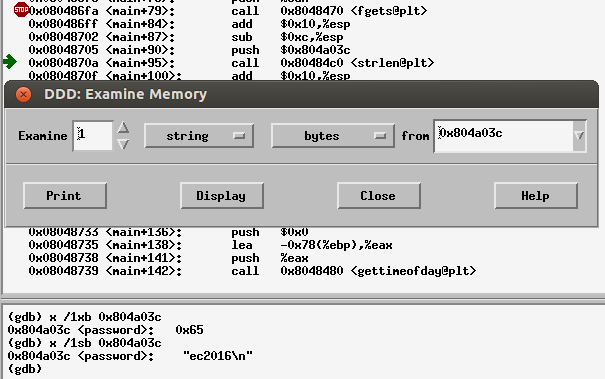
\includegraphics[scale=0.9]{capturas/figura1.png} 
	\caption{Examine Memory desde DDD} 
	\label{fig:figura1}
\end{figure}

Justo después del guardado de la contraseña introducida, se hace un \textbf{push} "sospechoso".
Ha sido el momento de examinar los datos en memoria mediante la opción \textbf{Data} $ \rightarrow $ \textbf{Memory}:

Poniendo Examine a 1, tipo \textbf{string} en \textbf{bytes} desde la dirección \textbf{0x804a03c} y haciendole un \textbf{print} ha mostrado la contraseña tal y como se ve en la Figura \ref{fig:figura1}.
\\

Contraseña: \textbf{ec2016}
\newpage

%----------------------------------------------------------------------------------------
%	
%----------------------------------------------------------------------------------------

\section{Código}
Para averiguar la contraseña se ha utilizado el depurador \textbf{DDD} realizando los siguientes pasos:
\\

Llegando a la sección del programa que se encarga de procesar y validar el código, se ha puesto un punto de ruptura en esta parte para futuros intentos.\\

Como se ve en la Figura \ref{fig:figura2} el programa hace una llamada a una función con nombre \textbf{desactivar}, por lo que mediante \textbf{stepi} la ejecución seguirá su curso adentrándose en ésta.\\
\begin{figure}[H]
	\centering
	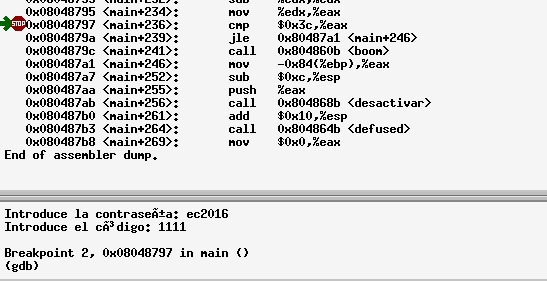
\includegraphics[scale=1]{capturas/figura2.png} 
	\caption{Examine Memory desde DDD para el código} 
	\label{fig:figura2}
\end{figure}
Una vez dentro de dicha función, tal y como se muestra en la Figura \ref{fig:figura3}, se pone un punto de ruptura para futuros intentos y a continuación se examina.


\begin{figure}[H]
	\centering
	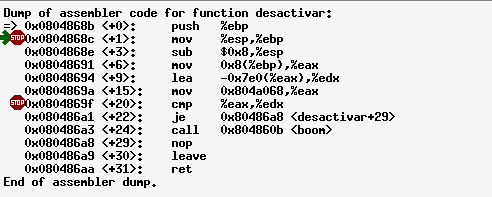
\includegraphics[scale=1]{capturas/figura3.png} 
	\caption{Examine Memory desde DDD para el código} 
	\label{fig:figura3}
\end{figure}

Mediante la ayuda del estado de los registros (\textbf{Status}$ \rightarrow $\textbf{Registers}) y avanzando una a una cada instrucción se puede ver cómo van modificando sus valores.
\newpage



El código de prueba introducido ha sido \textbf{1111}, sin embargo $ " $extrañamente$ " $ se ha visto cómo se ha modificado su valor convirtiéndose ahora en \textbf{-905}, como puede verse en la Figura \ref{fig:figura4}.

Es ahora cuando se hace una comparación de este nuevo valor con el valor que contiene \textbf{\%eax} que es cero.
\begin{figure}[H]
	\centering
	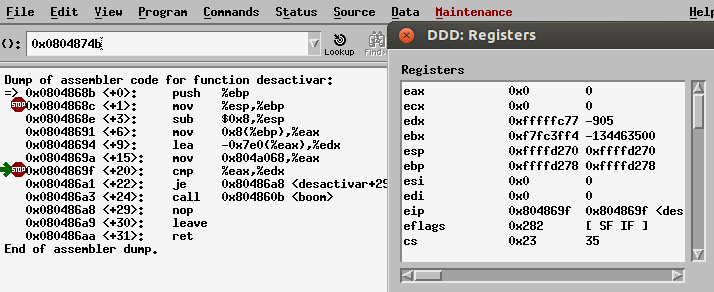
\includegraphics[scale=0.8]{capturas/figura4.png} 
	\caption{Examine Memory desde DDD para el código} 
	\label{fig:figura4}
\end{figure}
Aquí es cuando se aprecia que se ha realizado una resta sobre el valor introducido y que su resultado tiene que ser cero. Por lo que sumando el valor introducido como prueba (1111) y el resultado después de la modificación (905) aparece la solución al problema: 1111+905=2016
\\

Por tanto, el código es \textbf{2016}.

%----------------------------------------------------------------------------------------
%	Referencias
%----------------------------------------------------------------------------------------
%------------------------------------------------

\bibliography{citas} %archivo citas.bib que contiene las entradas 
\bibliographystyle{plain} % hay varias formas de citar

\end{document}
